\documentclass[nonumbib,leqno]{nrc1}
\usepackage{amssymb, amsmath, bm, epsfig,psfrag,graphicx}
\usepackage[french, english]{babel}
\usepackage{setspace}
\usepackage{lineno}
\usepackage{natbib}
\usepackage{longtable}
\usepackage{booktabs}
%added 9/29/08
%\usepackage[nolists]{endfloat}
\bibpunct{(}{)}{;}{a}{}{;}
\setlength{\mathindent}{1cm}

\setcounter{page}{1}
\volyear{XX}{201X}
\journal{Can. J. Fish. Aquat. Sci.}

\received{}

\bibliographystyle{ecology}

\begin{document}

\title{Assessing the detectability of prey removal effects on Steller sea lion ({\it Eumetopias jubatus}) abundance}

\author[P. B. Conn, D. S. Johnson, L. W. Fritz, B. S. Fadely]{Paul B. Conn, Devin S. Johnson, Lowell W. Fritz, Brian S. Fadely}
\address{National Marine Mammal Laboratory, Alaska Fisheries Science Center,
NOAA National Marine Fisheries Service,
Seattle, Washington, U.S.A. 98115}
\correspond{paul.conn@noaa.gov}

\shortauthor{Conn et al.}
\large

\maketitle

{\sc Running Head}: Prey removal and Steller sea lions \bigskip

May 13, 2013



\clearpage

\linenumbers

%% ABSTRACT %%%%%%%%%%%%%%%%%%%%%%%%%%%%%%%%%%%%%%%%%%%%%%%%%%%%%

%{\sc Summary.}
\begin{abstract}
\large
we'll do this last
%\keywords{}
\end{abstract}

%\begin{resume}
%\end{resume}

\keywords{Steller sea lions}


\clearpage

\renewcommand{\baselinestretch}{1.8}\normalsize


\section{Introduction}

1. Steller sea lion status relative to ESA, Western vs Eastern stock, decline proportion (from trend reports?)

2. Mitigation measures affect fisheries, lack of consensus on proximate causes of decline

3. Data at hand to assess relationship between fishing and Steller sea lion demography: adult \& pup,
A large number of studies have been conducted attempting to relate Steller sea lion abundance (pup counts, non-pup counts, `growth rate') to fishery variables (catch, No. hauls, CPUE [catch per tow]).  Results of these studies. Reasons why these data aren't ideal.  Inferences made from lack of significant results (i.e. Bernard et al. want to infer lack of relationship from lack of significant tests).



In this paper, we use simulation to investigate whether available SSL aerial survey metrics (adult or pup counts, count ratios) and explanatory variables commonly compiled from fisheries datasets are sufficient to reveal relationships between SSL population dynamics and prey availability. To conduct simulations, we consider the joint dynamics of SSL, a prey population, and a fishery.  A tacit assumption in all of our simulations is that sea lion dynamics depend on availability of the prey resource through one or more demographic component (e.g. fecundity, survival).  Due to data limitations and the complexity of simulated dynamics, our approach makes a number of simplifying assumptions (e.g. spatially independent populations, a single prey species).  However, these simplifications all serve to increase the power of detecting a relationship between fishing and SSL abundance; if we cannot do a good job of relating the two with simulated data, our case is even more hopeless in the real world!

The remainder of this article is structured as follows.  First, we describe a number of alternative models for the coupled fishery and SSL dynamics.  These models are intended to encompass a number of
alternative states of nature, including the functional relationship between sea lions and fish, as well as
how fishing effort is allocated (i.e., whether or not it is dependent on fish distribution).  Next, we provide details on how we calibrated these models to generate reasonable parameter estimates for simulation.  We then describe our overall simulation structure and provide details on the simulation outputs (e.g., conventional test statistics, Bayesian model weights) that we used to measure our ability to detect relationships between SSL abundance and explanatory fisheries variables.  After describing results, we conclude by offering some final thoughts about how best to interpret SSL-fisheries interactions on the base of available data.


\section{Methods}

We considered models for coupled dynamics between fishers, fish, and SSL, where fish and SSL were modeled as island populations (i.e. assuming independent dynamics among islands).  In reality, there are substantial dispersal of SSL among rookery and haulout areas.  Similarly, relevant fish populations in the Gulf of Alaska and Bering Sea (e.g., Atka mackerel, pacific cod, walleye pollock) are interconnected through movement and recruitment processes.  However, the assumption of independent dynamics should provide greater power for detecting meaningful relationships between SSL aerial survey counts and fishery variables since responses of SSL to experimental treatments (fishing) are not blurred by uncontrollable and poorly understood processes.  Thus, a simulation design assuming island populations should provide a useful one-way test for whether the approach of relating fishery variables to SSL counts provides reasonable inferences.

\subsection{Models}


To induce coupled dynamics between SSL, fish, and fishers, we modeled
fish mortality as a function of both fishing effort and SSL predation, where annual fish recruitment follows a Beverton-Holt spawner-recruit function \citep{Beverton1957} with lognormal error (separate models for state dynamics are modeled for each island population).  In turn, we made SSL dynamics dependent on the expected per capita number of fish ``harvested" by SSL, where dependency can be expressed in terms of survival or fecundity (depending upon simulation configuration).  Finally, we considered two scenarios for fisher dynamics, allowing fishing effort to be (i) randomly allocated each year, or (ii) allocated in proportion to fish biomass in each island population.  Each of these components are described in further detail below.


\subsubsection{Steller sea lion model}

We based SSL dynamics loosely on the age-structured, (`HFYS') Leslie-matrix model described by \citet{HolmesEtAl2007}, who summarized fecundity and survival probability for SSL for ages $0-30$ (survival probability was assumed zero after age 30).  This model assumes a post-breeding census, coinciding with annual aerial surveys of rookeries and haul-outs in the Gulf of Alaska and Aleutian islands in June and July.  As presented, this `base' Leslie-matrix has a dominant eigenvalue of 1.000, which is indicative of a stable population (at least in absence of demographic stochasticity).

To make SSL demography dependent on the number of fish, we allowed either female fecundity at age ($f_{a,t,k}$) or female survival at age ($S_{a,t,k}$) (Table \ref{tab:model}) to be dependent on the ratio of fish to sea lion biomass.  Survival probability is naturally bounded in the $(0,1)$ interval, while
fecundity is biologically constrained to be in the $(0,1)$ interval (females usually produce a maximum of one pup per year), so we model both parameters on the logit scale:
\begin{linenomath}
\begin{equation*}
{\rm logit}(S^f_{a,t,k})=\alpha_{0,a} + \alpha_1 B_{t,k}^*/X_{t,k} \hspace{2mm} {\rm or}
\end{equation*}
\end{linenomath}
\begin{linenomath}
\begin{equation*}
{\rm logit}(f_{a,t,k})=\beta_{0,a} + \beta_1 B_{t,k}^*/X_{t,k}.
\end{equation*}
\end{linenomath}
Here, $S^f_{a,t,k}$ gives survival of female age $a$ SSL in year $t$ of simulation for site $k$, $f_{a,t,k}$ gives SSL fecundity for age $a$ in year $t$ and site $k$, $B_{t,k}^*$ gives SSL biomass in year $t$ in site $k$, and $X_{t,k}$ gives fish biomass that is exploitable by SSL in year $t$ and site $k$ (for a complete list of notation, see Table \ref{tab:model}).  We modeled male SSL dynamics by assuming a 50/50 sex ratio at age 0, and a fixed ratio $r_a$ between female and male survival thereon (i.e., $S^m_{a,t,k}=r_a S^f_{a,t,k}$).  We calculated $r_a$ using the ratio of male to female ``CP" survival estimates reported in appendix C of \citet{HolmesEtAl2007}. Biomass of both sexes was calculated using Richards growth curves (DEVIN, HELP - also see biomass entry in notation table). We calibrate parameters describing the hypothetical relationship between demographic parameters and relative biomass of SSL and prey at the start of year $t$ ($\alpha_0,\alpha_1,\beta_0,\beta_1$) in a later section (see \ref{section:Calibration}).

\subsubsection{Prey (fish) model}

A variety of commercially important fish stocks are affected by time-area closures designed to protect SSL, most notably walleye pollock ({\it Theragra chalcogramma}), pacific cod ({\it Gadus macrocephalus}), and Atka mackerel ({\it Pleurogrammus monopterygius}).  Rather than base fish dynamics on just one (or multiple) of these species, we modeled fish dynamics of a hypothetical, generic species that combined similar life history and exploitation features from each stock.  For simplicity, we use the same annual time step for the fish population as for SSL, modeling recruitment as occurring immediately prior to annual aerial surveys.  An age-structured population dynamics model was assumed for each simulated fish stock, with 10 ages (1-9 and 10+).
We write total mortality rate for a given fish age class $a$ at time $t$ at site $k$ as $Z_{a,t,k}=M + F_{t,k}^* + F_{a,t,k}$, where $M$ gives
natural mortality, $F_{t,k}^*$ gives a mortality rate attributable to SSL in site $k$ in year $t$ of simulation, and $F_{a,t,k}$ gives time- and age-specific fishing morality (recall that notation is also defined in Table \ref{tab:model}).  Recent assessments of walleye pollock, pacific cod, and Atka mackerel stocks \citep[e.g.][]{PollockAssessment2011,PacCodAssessment2011,AtkaAssessment2012} indicated natural mortality rates in the 0.3-0.34 range.  However, these figures include all natural mortality, including SSL predation (which we model separately).  For our hypothetical fish stock, we set $M=0.2$ during simulations.

We modeled fishing mortality, $F_{a,t,k}$, as a product of an age-specific selectivity curve and a fully selected fishing mortality rate that is itself a function of fishing effort, such that $F_{a,t,k}=q E_{t,k} s_a$, where $E_{t,k}$ summarizes fishing effort for site $k$ in year $t$, $s_a$ describes selectivity at age, and $q$ is a catchability coefficient.  Recent assessments of fish stocks in the Bering sea used flexible selectivity functions that were allowed to evolve over time; these pointed to dome-shaped selectivity functions in the majority of cases.  For simulations, we used a dome-shaped double logistic model constructed so as to approximate the general shape obtained in the assessments (Fig. \ref{fig:at_age}, Table \ref{tab:model}).  For further description of effort and catchability, we refer the reader to subsequent sections \ref{section:Fleet} and \ref{section:Calibration}, respectively.

For SSL-related mortality, we imposed a model of the form $F_{a,t,k}^*=\delta s_a^* N_{t,k} B_{t,k}^*$, where $s_a^*$ gives the relative selectivity of SSL on age $a$ fish, $N_{t,k}$ gives the total number of fish in population $k$ at time $t$, $B_{t,k}^*$ gives the SSL biomass at time $t$, and $\delta$ gives a capture efficiency parameter. This is a similar functional form as used in classic Lotka-Volterra predator-prey models \citep[see e.g.][]{Gotelli2001}, with the modification that we use biomass (instead of numbers) of SSL to allow for the fact that larger sea lions will likely consume more fish than smaller ones.  Once again, we leave it until a later section (\ref{section:Calibration}) to determine reasonable values for $\delta$.

\citet{ZeppelinEtAl2004} reported substantial overlap between sizes of walleye pollock and Atka mackerel harvested by SSL and commercial trawl fisheries, although the distribution of fish lengths selected by SSL was shifted to the left (i.e., towards smaller-sized fish).  SSL selectivity likely varies by a number of factors, including year, SSL size/age, fish availability, and location \citep{ZeppelinEtAl2004}.  For our simulation study, we constructed a double logistic selectivity that was offset from fishery selectivity to have a modal age that was two years less (Fig. \ref{fig:at_age}, Table \ref{tab:model}).

Annual recruitment at each site was modeled using a Beverton-Holt spawner-recruit curve subject to lognormal error.  A popular parameterization of this model is
\begin{linenomath}
\begin{equation*}
N_{1,t+1,k} = \frac{0.8 R_{0,k} h SSB_{a,t,k}}{0.2 \phi_0 R_{0,k}(1-h)+(h-0.2)SSB_{t,k}} \exp{\epsilon_{t,k}},
\end{equation*}
\end{linenomath}
where $N_{1,t,k}$ gives the number of recruits (age 1 individuals) in year $t$ at site $k$, $R_{0,k}$ is expected annual recruitment in absence of fishing (allowed to be different across sites), $SSB_{t,k}$ gives spawning biomass in year $t$, $h$ is steepness, $\phi_0$ is unfished spawning biomass per recruit (calculated in absence of SSL), and $\epsilon_{t,k}$ represents Gaussian noise \citep{Mace1988}.  Spawning stock biomass can be calculated from knowledge of numbers of fish in each age class, together with maturity at age and weight at age vectors (Table \ref{tab:model}).

\subsubsection{Fleet dynamics}
\label{section:Fleet}

We considered two scenarios for fleet dynamics, both of which assume that total fishing effort stays constant
over the course of simulation time (at least in portions of simulation time series where fishing occurs).  In the first scenario, we allow fishing effort to be annually redistributed according to a ${\rm Dirichlet}(1,1,\hdots,1)$ distribution.  This formulation approximates the situation where experimental treatments (fishing) are applied randomly to experimental units (sites).  As such it is clearly unrealistic, as fishing vessels will likely try to optimize catch by going to areas where there are more fish, perhaps subject
to economic and time constraints (e.g., distances from port).  Nevertheless, this scenario likely provides the greatest power to detect relationships between SSL survey counts and fishing variables.

Our second scenario assumes that fishing fleets redistribute effort each year according to the exploitable biomass of fish at each site.  This scenario is also clearly unrealistic, as it assumes fishers have omniscient knowledge about the distribution and abundance of fish, and no economic constraints influencing their movements (e.g. fuel costs, time).  However, this distribution of effort represents an ideal free distribution \citep{FretwellLucas1970}, which has a rich use in ecology.  It also represents the opposite end of the spectrum from the first scenario, where there was no relationship between fishing effort and fish abundance.

For each scenario, we calculated catch at each site using the Baranov catch equation \citep{Baranov1918}; see Table \ref{tab:model}.


\subsubsection{Survey models/measurement error}

We investigate the case where $K=37$ sites are surveyed by annual SSL aerial surveys that count the total
number of non-pups (age 1+).  We also simulated annual SSL pup surveys. Aerial survey counts are an imperfect measure of abundance for two reasons.  First, not all animals are present on haul-outs or rookeries when surveys are conducted, because some proportion are out foraging.  Second, survey counts are subject to measurement error (not all animals present are counted).  \citet{HolmesEtAl2007} investigated the variability of counts from repeat aerial surveys of adults that were conducted in the same year, and suggested that the coefficient of variation (CV) for these counts was $\approx 5\%$.  We used this value to induce lognormal measurement error on observed non-pup counts, assuming that
\begin{linenomath}
  \begin{equation}
     I_{t,k} = p N_{1+,t,k}^{*}\exp{\epsilon_{t,k}},
  \end{equation}
\end{linenomath}
where $I_{t,k}$ gives the non-pup survey count at site $k$ at time $t$, $N_{1+,t,k}^*=\sum_{a=1}^{30} N_{a,t,k}^{*f}+N_{a,t,k}^{*m}$ gives non-pup SSL abundance (see Table \ref{tab:model}), and $\epsilon_{t,k}$ gives mean zero Gaussian distributed noise with standard deviation set to the desired CV of 0.05. We acknowledge that the small CV of 0.05 understates likely variation in the relationship between survey counts and underlying abundance; for instance, the portion of animals available for sampling each year may change if the time spent foraging changes (e.g., in responses to prey abundance).  Nevertheless, our approach is consistent with the goal of maximizing power to detect prey removal effects on SSL abundance.

We also simulated surveys of SSL pups, where generated pup counts were simulated from a binomial distribution with success probability 0.95:
\begin{linenomath}
  \begin{equation}
     P_{t,k} \sim {\rm Binomial}(N_{0,t,k}^*,0.95).
  \end{equation}
\end{linenomath}
In this case, we assumed that all pups would be available for detection (hauled out), but we allowed for 5\% to be missed on average (due to visual obstruction, for example).

\subsection{Simulation design}

We used a $2 \times 2$ factorial simulation design that included design points for each combination of fleet effort allocation (random or proportional to fish abundance) and SSL demographic component (whether fecundity or survival was related to prey availability).  For each design point, we conducted 5000 simulations, each of which had a similar overall design (Fig. \ref{fig:sim_diagram}).
In each simulation, we randomly generated virgin fish recruitment ($R_{0,k}$) at each of $K=37$ sites (the approximate number of rookeries for the western SSL stock), and initialized prey and SSL abundance according to their stable age distributions \citep[cf.][]{Caswell2001}.  \citet{LoughlinEtAl1992} suggested a population of 240,000-300,000 in the 1950s; we therefore initialized SSL abundance at 250,000, divided equally among sites, at the beginning of each simulation.  We then simulated dynamics of SSL and prey for 150 years in absence of fishing, a time period which allowed SSL abundance to stabilize with the number of prey available.  This approach also induced stochasticity in the age structure of both species (resulting from annual fish recruitment variation).  We then introduced fishing, and aerial surveys were simulated beginning 25 years later (these were conducted for the next 20 years of simulation time).  These time periods were selected to approximate the introduction of fishing pressure and the institution of consistent aerial SSL surveys in the Bering Sea and Gulf of Alaska; for relevant fish stocks (e.g. Alaska pollock), heavy commercial fishing began in the mid-late 1960s. The first aerial surveys began in 1976, but consistent survey effort was not obtained until the early 1990s.  The survey collection period of 20 years approximates data collection for 1991 through 2010.

Following each simulation, we attempted to test whether SSL counts ($I_{t,k}$ or $P_{t,k}$) or measures of change in counts ($\lambda_{t+1,k}^{1+}=I_{t+1,k}/I_{t,k}$ or $\lambda_{t+1,k}^{0}=P_{t+1,k}/P_{t,k}$ , were related to fishing variables ($E_{t,k}$,$L_{t,k}$,$U_{t,k}$) in the previous year.  To test for such relationships, we fit a sequence of generalized linear mixed pseudo-models \citep[GLMPM;][]{VerHoef2010} to each simulated data set.  Previous analyses reported in the literature sometimes accounted for site-specific differences using mixed models \citep{Hui2011}, or temporal autocorrelation via generalized estimating equations \citep{Dillingham:2006fv,Trites:2010ly}, but never both.  The GLMPM framework is an improvement in this regard, as it uses random effects to account for differences in responses among sites, and accounts for autocorrelation via an AR1 structure.  For our purposes, count-level responses (i.e., $I_{t,k}$, $P_{t,k}$) were modeled using a Poisson error structure, while continuous responses (i.e., $\lambda_{t,k}^{0}$, $\lambda_{t,k}^{1+}$) were modeled with a Gaussian error structure.  For each combination of response and predictor variable, we used the \texttt{glmmLDTS} package \citep{VerHoef2010} within the R programming environment \citep{RDevelopmentCoreTeam2012} to fit a separate GLMPM model including both an intercept and a linear effect of the predictor. For each such model, we recorded both the sign of the estimated slope coefficient (indicating whether the effect on SSL was positive or negative), as well as the associated p-value.

\subsection{Calibration}
\label{section:Calibration}

Several simulation inputs (Table \ref{tab:inputs}) required a calibration exercise to determine reasonable values prior to simulation.  These included parameters describing SSL fecundity as a function of prey availability ($\alpha_0$ and $\alpha_1$), those describing SSL survival as a function of prey availability ($\beta_0$ and $\beta_1$), capture efficiency of SSL ($\delta$), and fish catchability associated with fishing effort ($q$).  We used simulated annealing \citep{Belisle1992}, as implemented in the R function \texttt{optim}, to obtain values of these parameters that best minimized an objective function representing several desired features of resulting time series.  In particular, we penalized time series whenever (1) simulated SSL numbers differed from any of 6 reconstructed SSL population estimates \citep[see][Table 1]{Goodman2008} (2) when mean fishing mortality rate across sites differed from 0.3 (for years where fishing occurred), and (3) when mean fish mortality rate attributable to SSL differed from 0.1.  In addition, we strongly penalized parameter values that resulted in SSL depletion below 0.05 in the 185th year of simulation (Table \ref{tab:objfun}). Recall that simulations were run for 195 years, approximating surveys up to 2010.  Separate sets of parameter values were calibrated depending on whether SSL survival or fecundity was linked to fish biomass.

\subsection{Posterior evidence}

Our simulation analysis is intended to summarize how well different types of fisheries and aerial survey data perform in illuminating functional relationships between SSL and prey, at least under idealized survey conditions.  A related question particularly relevant for SSL management is the degree to which the outcome of a statistical test (e.g., significantly positive, significantly negative, or no effect) should be used to update a manager's prior beliefs as to the effect of fisheries on SSL populations.  For instance, assume that a manager has three working hypotheses: 
\begin{itemize}
\item $M_1$: SSL vital rates do not depend on prey biomass
\item $M_2$: SSL survival depends on prey biomass, or
\item $M_3$: SSL fecundity depends on prey biomass,
\end{itemize}
and that they are willing to assign a prior probability mass, $Pr(M_i)$ to each hypothesis.  For instance, 
they might choose $Pr(M_i)=1/3$ to give equal weight to each working hypothesis before examining the results of any statistical test.

For the moment, assume that one of the models we have introduced to describe SSL-fish-fishery interactions and population surveys is a reasonable depiction of underlying dynamics.  In this case, standard application of Bayes' rule can be used to update the probability of each working hypothesis given (1) a statement of significance from a real life statistical test, and (2) simulation results describing the proportion of simulations that resulted in significantly positive, significantly negative, or statistically insignificant tests.  Specifically, the updated probability associated with working hypothesis $M_i$ is given by
\begin{linenomath}
  \begin{equation}
     \label{eq:Bayes}
     Pr(M_i | {\rm Data}) = \frac{Pr({\rm Data}|M_i)Pr(M_i)}{\sum_j Pr({\rm Data}|M_j)Pr(M_j)}.
  \end{equation}
\end{linenomath}
For each simulation scenario and choice of dependent and independent variables, we use Eq. \ref{eq:Bayes} to calculate the posterior probability of each working hypothesis under a hypothetical real world test result, replacing $Pr({\rm Data}|M_i)$ with empirical estimates from our simulation study.  For instance, if we wish to update the posterior probability of model $M_i$ given a hypothetical real world test result of ``not significant," we simply replace $Pr({\rm Data}|M_i)$ with the proportion of simulation runs for which working hypothesis $i$ resulted in a statistically insignificant test.  Since we did not run any simulations for working hypothesis $M_1$, we assume nominal error rates (i.e., we specified that 2.5\% of tests would result in significantly positive and significantly negative statistical tests in the case that vital rates do not depend on prey biomass).

\section{Results}

Our calibration exercise resulted in time series that largely captured desired features (Fig. \ref{fig:sim_trajectories}).  Depending upon input configuration, fishing mortality averaged 0.30-0.32 (recall our target was 0.30), and fish mortality attributable to SSL averaged 0.069-0.074.  (recall our target was 0.1).  After initialization, realized time series for SSL took 50-100 years to stabilize.  Introduction of fishing at the 150th year of simulation led to marked decreases in fish abundance and SSL abundance, albeit at levels of depletion not as severe as those exhibited in actual SSL numbers.

\section{Discussion}

In this paper, we asked a relatively simple question: given a simulated population that strongly resembles the western SSL stock, are we able to relate SSL survey data to fishery variables when SSL vital rates are tied to prey availability? Our investigation suggests that one is unlikely to detect a negative effect between non-pup abundance and fishery variables even under ideal conditions - including independence among site level responses (induced by simulating island populations), random application of treatments (fishing) to experimental units (sites), and annual sampling.  This finding is particularly disconcerting in our case because data were simulated such that SSL population declines were ultimately attributable to fishing.

On the other hand, tests relating SSL pup survey data to available fishery variables suggested that available state variables (e.g. fishery CPUE, pup survey counts) should provide ample power to detect whether SSL fecundity is related to prey availability, at least under the idealized study conditions assumed here.


departures from ideal conditions - nonrandomness, etc.

To date, the most comprehensive analyses addressing SSL declines have largely implicated decreases in recruitment as a likely reason for non-recovery of the western stock.  For instance, \citet{HolmesEtAl2007} estimated the life history components that would need to be reduced to result in
the patterns of observed population decline exhibited in SSL datasets from 1976-2004.  They found support for a model with a sudden, albeit temporary drop in non-pup survival in the early 1980s coupled with an overall decrease in birth rates.  This finding implicates reduced non-pup survival in the initial crash of SSL; however, chronic depression in birth rates appears to be the primary reason why SSL stocks have not recovered.  Similarly, \citet{Wolf:2008qf} fit alternative models encompassing several different working hypotheses about SSL decline, and found strong support for models where recruitment was written as a function of total prey availability or prey species composition.

Our inability to relate SSL non-pup abundance and one year growth rates to fishery variables is perhaps not surprising.  Even through prey abundance was largely responsible for SSL declines in our simulations, fishery variables provided noisy depictions of prey abundance (at best).  Further, it is well known that long lived species exhibit strong momentum in population dynamics \citep[see][for a review]{EzardEtAl2010}, where perturbations (e.g., changes in survival, fecundity) can take many years to fully manifest themselves.  As such, changes in short term abundance or population growth reflect not only the present set of demographic parameters, but changes in those parameters that occurred years in the past.  Thus there is a subtle mismatch between the time scales of the dependent and independent variables.

Our point in this paper is not to advocate a particular position regarding the ultimate effects of fishing on SSL populations.  To our mind, the reason for SSL decline (and lack of recovery) is still an open question with several possible explanations (e.g., reduced prey availability, a shift in the relative composition of prey abundance, increase in killer whale predation, or some combination thereof).  Our results simply indicate that a lack of statistical significance in previous studies cannot be used as credible scientific evidence against the prey availability hypothesis, at least as far as adult survival is concerned.  Our results do suggest the possibility for relating recruitment (via pup counts) to fishery variables.  However, further study would be needed to determine the power of such tests under more realistic sampling conditions (e.g., reduced frequency of surveys, lack of randomization, lack of independence among fish and SSL populations, etc.).

A recent review \citep{Bernard:2011dq} suggested that a lack of statistically significant negative effects in published literature provides evidence that high value fisheries for pollock, Atka mackerel, cod do not negatively impact SSL populations.  By contrast, our study shows that many of these studies, no doubt carried out with the best of intentions, have little to no power to provide meaningful inferences regarding the prey limitation hypothesis.  In addition to the basic inferential problem involved with selecting meaningful dependent and independent variables (as exhibited by our results), these studies are further many of these studies used statistical methods that

suggestions: use GLMPMs, focus on pups with aerial data, try to get adult survival estimates (photogrammetry), better characterize available exploitable prey biomass, adaptive management (whooping cranes).


\bibliography{SSLfish_biblio}

\begin{longtable}{p{4cm}lll p{8cm}}
\caption[Population \& Fisheries dynamics]{\large Notation and dynamical equations used to simulate
 hypothetical Steller sea lion (SSL), fish, and fisheries data.} \label{tab:model} \\
%\begin{tabular}{p{4cm}lll p{8cm}}
\hline \hline
Quantity & & Symbol & & Description or definition \\
\cline{1-1} \cline{3-3} \cline{5-5} \\
\endfirsthead
\hline \hline
Quantity & & Symbol & & Description or definition \\
\cline{1-1} \cline{3-3} \cline{5-5} \\
\endhead
\hline
\endfoot
\hline
\endlastfoot
\multicolumn{1}{l}{\textbf{Steller sea lion dynamics}}\\
Female survival & & $S_{a,t,k}^f$ & & Probability of age $a$ SSL survival for females from year $t$ to year $t+1$ at site $k$, where

$\textrm{logit}(S_{a,t,k}^*)=\alpha_{0,a}+\alpha_1 B_{t,k}^*/X_{t,k}$.

Note that $S_{31,t,k}^*=0$ so there is no plus group.\\
Male survival & & $S_{a,t,k}^{m}$ & & $S_{a,t,k}^{m}=r_a S_{a,t,k}^f$.  \\
Fecundity & & $f_{a,t,k}$ & & Expected number of female pups per age $a$ SSL female in year $t$ at site $k$,
given as

$\textrm{logit}(f_{a,t,k})=\beta_{0,a}+\beta_1 B_{t,k}^f/X_{t,k}$. \\
Initial abundance & & $N_{init}$ & & Total abundance of SSL at the beginning of simulations.  Set to 250,000 in all simulations \\
Leslie matrix & & $\textbf{A}$ & & SSL Leslie matrix formed from survival and fecundity parameters when $\alpha_1$ and $\beta_1$ are set to zero; used to set initial age distribution at start of simulations \\
Initial age proportion & & $\pi_{a,s}$ & & Proportion of population that is of age $a$ and sex $s$ at the beginning of simulations (set using Leslie matrix theory) \\
Numbers at age & & $N_{a,t,k}^f$,$N_{a,t,k}^{m}$ & & Number of age $a$ female (male) SSL during surveys in year $t$ at site $k$.  Initial age structure is set for females as $N_{a,1,1}^f=\pi_{a,1}N_{init}/K $ and $N_{a,1,2}^m=\pi_{a,2}N_{init}/K $ for males.  For subsequent years ($t>1$),

$N_{0,t+1,k}^f \sim {\rm Poisson}(\sum_a N_{a,t,k}^ff_{a,t,k})$,

$N_{t+1,k}^f \sim {\rm Binomial}(N_{a,t,k}^f,S_{a,t,k}^f)$,

${\bf N}_{0,t+1,k}^{m} {\rm Poisson}(\sum_a N_{a,t,k}^f f_{a,t,k})$, and

$N_{t+1,k}^{m} \sim {\rm Binomial}(N_{a,t,k}^{m},S_{a,t,k}^{m})$. \\
Initial
Biomass at age & & $B_{a,t,k}^f,B_{a,t,k}^{m}$ & & Biomass of age $a$ female (male) SSL during surveys in year $t$ at site $k$; calculated as DEVIN, HELP (maybe put growth parameters in table 2?)\\
Total biomass & & $B_{t,k}^*$ & & Total SSL biomass at site $k$ during surveys in year $t$ ($B_{t,k}^*=\sum_a B_{a,t,k}^f+B_{a,t,k}^{m}$) \\
\midrule
\multicolumn{1}{l}{\textbf{Fish dynamics}}\\
Weight-at-age & & $w_a$ & & $w_a = [ 1 + \exp(-b^{\rm wgt}(a-a_{50}^{wgt})) ]^{-1}$ \\
Maturity-at-age & & $m_a$ & & $m_a = [ 1 + \exp(-b^{\rm mat}(a-a_{50}^{mat})) ]^{-1}$ \\
Unfished spawning biomass per recruit & & $\phi_0$ & & $\phi_0=\sum_{a=1}^9 \{ \exp(-aM) w_a m_a \} + \frac{\exp(-10M) w_{10} m_{10}}{1-\exp(-M)}$ \\

Fishery selectivity  & & $s_a$ & &  $s_a = \frac{1}{1+\exp(-\eta_1(a-\kappa_1))} \left( 1- \frac{1}{1+\exp(-\eta_2(a-\kappa_2))} \right)$ (rescaled to have a maximum of 1.0)\\

Fishery mortality rate & & $F_{tk}$ & & $F_{tk}=q E_t$, Fully selected fishing mortality rate for year $t$, site $k$\\

Fishing mortality rate at age & & $F_{a,t,k}$ & & $F_{a,t,k}=s_a F_{t,k}$ \\

SSL selectivity  & & $s_a^*$ & &  $s_a^* = \frac{1}{1+\exp(-\eta_1^*(a-\kappa_1^*))} \left( 1- \frac{1}{1+\exp(-\eta_2^*(a-\kappa_2^*))} \right)$ (rescaled to have a maximum of 1.0)\\

SSL predation rate  & & $F_{t,k}^*$ & & $F_{t,k}^*=\delta N_{t,k} B_{t,k}^* s_a^*$ \\

Natural mortality rate & & $M$ & & Assumed constant (0.2) for all simulations \\

Total mortality rate at age & & $Z_{a,t,k}$ & & $Z_{a,t,k}=M+F_{a,t,k}+F_{a,t,k}^*$ \\[2pt]
\\

Abundance at age & & $N_{a,t,k}$ & & $N_{1,1,k} = R_{0,k}$ \newline
$N_{a+1,1,k}=N_{a,1,k}\exp(-Z_{a,1,k})~~~\forall a \in (1\ldots 9)$ \newline
$N_{10,1,k}=N_{9,1,k} \frac{\exp( -Z_{9,1,k})} {1-\exp (-Z_{10,1,k})}$ \newline
$N_{1,t+1,k}=\frac{0.8 R_{0,k} h SSB_{t,k}} {0.2\phi_0 R_{0,k} (1-h)+(h-0.2)SSB_{t,k}}
  \exp(\epsilon_{t,k}^R)$ \newline
$N_{a+1,t+1,k}=N_{a,t,k}\exp(-Z_{a,t,k})~~~\forall a \in (1\ldots 9)$ \newline
$N_{10,t,k}=N_{10,t-1,k} \frac{\exp( -Z_{9,t-1,k})}{1-\exp (-Z_{10,t-1,k})}$ \newline
where $\epsilon_{t,k}^R \sim {\rm Normal}(0,\sigma_R)$, $\phi_0$ gives unfished spawning biomass per recruit, and $h$ gives steepness (set to 0.8).  \\[2pt]

Total abundance by site & & $N_{t,k}$ & & $ \sum_a N_{a,t,k}$ \\

Spawning biomass & & $SSB_{t,k}$ & & $SSB_{t,k}=\sum_a N_{a,t,k} w_a m_a$ \\

Exploitable biomass (to fishery) & & $B_{t,k}$ & & $B_{t,k}= \sum_a N_{a,t,k} w_a s_a$\\

Exploitable biomass (to SSL) & &  $X_{t,k}$ & & $X_{t,k}= \sum_a N_{a,t,k} w_a s_a^*$\\

\midrule

\multicolumn{1}{l}{\textbf{Fleet dynamics}}\\

Fishing effort (random) & & $E_{t,k} $ & & $ E_{t,k} \sim {\rm Dirichlet}(1,1,\hdots,1)$ \\[2pt]

Fishing effort (directed) & & $E_{t,k}$ & & $ E_{t,k} = B_{t,k}/\sum_{k} B_{t,k} $, \newline \\[2pt]

Catchability & & $q$ & & Relates fishing mortality rate to effort (see $F_{t,k}$ definition) \\

Catch-at-age & & $C_{a,t,k}$ & & Calculated with Baranov catch equation: $C_{a,t,k}=F_{a,t,k}/Z_{a,t,k} (1-\exp(-Z_{a,t,k}) N_{a,t,k}$ \\

Catch (numbers) & & $C_{t,k}$ & & $C_{t,k}=\sum_a C_{a,t,k}$ \\

Catch (weight) & & $L_{t,k}$ & & $L_{t,k}=\sum_a C_{a,t,k} w_a$ \\

CPUE Index & & $U_{t,k}$ & & $U_{t,k} \sim {\rm lognormal}(\log(L_{t,k}/E_k),\sigma^2)$, where $\sigma=\sqrt{log(0.2^2+1)}$ (implying a CV of 0.2) \\

\midrule

\multicolumn{1}{l}{\textbf{Aerial survey data}}  \\
Non-pup survey count  & & $I_{t,k}$ & & Count of non-pup (age 1+) SSL during the simulated aerial survey of site $k$ at time $t$\\
Pup survey count  & & $P_{t,k}$ & & Count of SSL pups during the simulated aerial survey of site $k$ at time $t$\\
\bottomrule
%\end{tabular}
\end{longtable}

\begin{table}
\caption{\setstretch{2} \large Definitions and values for simulation input variables.  The subscript $\dag$
indicates values that were fixed as an outcome of calibration exercises; remaining simulation inputs were
set a priori.}
\label{tab:inputs}
\begin{tabular}{p{3cm}lll p{9cm}}
\\
\hline \hline
Input variable & & Value & & Definition\\
\cline{1-1} \cline{3-3} \cline{5-5}
\\
\multicolumn{1}{l}{\textbf{Survey variables}}  \\
$Y_1$ & & 100 & & Number of simulation years with just SSL (no fishing) \\
$Y_2$ & & 10 & & Number of years of fishing before aerial surveys begin \\
$Y_3$ & & 30 & & Number of years with both fishing and simulated aerial surveys \\
$K$ & & 37 & & Number of ``sites" (SSL populations)  \\
$\sigma_I$ & & 0.05 & & Coefficient of variation (CV) for aerial survey counts \\
\midrule
\multicolumn{1}{l}{\textbf{SSL variables}}  \\
$p$ & & 0.5 & & Proportion of adult SSL available (hauled out) during aerial surveys \\
$r_a$ & & see Fig. & & Fixed ratio
of male to female survival at age from \citet{HolmesEtAl2007}, Appendix C. \\
$\alpha_{0,a}$ & & $=\alpha_0 \nu_a $ & & Intercept of SSL survival model (logit scale) \\
$\alpha_0$ & & $3.38,2.76^\dag$ & & Scaling parameter for the intercept of the SSL survival model used in
                                    survival and fecundity simulations, respectively\\
$\nu_a $ & & $\log(S_a/(1-S_a))$ & & Base age $a$ SSL female survival value on the logit scale (setting $S_a$ to the HFYS female survival values reported by \citet{HolmesEtAl2007})  \\
$\alpha_1$ & & $-9.02^\dag$ & & Slope parameter of SSL survival model controlling per capita dependence on prey abundance.  This parameter was set to 0.0 in fecundity simulations. \\
$\beta_{0,a}$ & & $\beta_0 \omega_a$ & & Intercept of SSL fecundity model (logit scale) \\
$\beta_0$ & & $2.01,1.28^\dag$ & & Scaling parameter for the intercept of the SSL fecundity parameter used in survival and fecundity simulations, respectively \\
$\omega_a$ & & $\log(f_a)$ & & Base age $a$ SSL fecundity value on the log scale (setting $f_a$ to the HFYS fecundity value reported by \citet{HolmesEtAl2007}) \\
$\beta_1$ & & $-3.89^\dag$ & & Slope parameter of SSL fecundity model; controls per capita dependence
                    on prey abundance.  This parameter was set to 0.0 for survival simulations \\
$\delta$ & & $1.33E-14,1.97E-15^\dag$ & & Capture efficiency parameter describing the rate at which SSL/fish encounters result in fish mortality (such that $F_{t,k}^*=\delta N_{t,k} B_{t,k}^*$).  Values are for survival and fecundity simulations, respectively. \\
\midrule
\multicolumn{1}{l}{\textbf{Fish variables}}  \\
$M$ & & 0.2 & & Natural mortality rate (in absence of SSL) \\ [2pt]
$R_{0,k}$ & & U(1000000,5000000) & & Virgin recruitment at site $k$; drawn from a uniform distribution at the beginning of each simulation \\
$h$ & & 0.8 & & Beverton-holt steepness \\
$\sigma_R$ & & 0.5 & & Standard deviation for lognormal recruitment deviations \\
$a_{50}^{\rm mat}$ & & 5 & & Age at 50\% sexual maturity \\
$b^{\rm mat}$ & & 1 & & Slope parameter for logistic maturity-at-age function \\
$a_{50}^{\rm wgt}$ & & 5 & & Age at 50\% weight \\
$b^{\rm wgt}$ & & 0.7 & & Slope parameter for logistic weight-at-age function \\
$\eta_1$ & & 1.3 & & Slope of ascending limb of double logistic selectivity curve (fishery)\\
$\eta_2$ & & 1 & & Slope of descending limb of double logistic selectivity curve (fishery) \\
$\kappa_1$ & & 4 & & Age at 50\% fishery selectivity (ascending) \\
$\kappa_2$ & & 10 & & Age at 50\% fishery selectivity (descending) \\
$\eta_1^*$ & & 1.3 & & Slope of ascending limb of double logistic selectivity curve (SSL) \\
$\eta_2^*$ & & 1 & & Slope of descending limb of double logistic selectivity curve (SSL) \\
$\kappa_1^*$ & & 2 & & Age at 50\% SSL selectivity (ascending) \\
$\kappa_2^*$ & & 8 & & Age at 50\% SSL selectivity (descending) \\
$ q $ & & $11.80,11.02^\dag$ & & Catchability coefficient relating fishery effort ($E_{a,t,k}$) to apical fishing mortality.  Values are for survival and fecundity simulations, respectively \\
\bottomrule
\end{tabular}
\vspace{4in}
\end{table}

\begin{table}
\caption{\setstretch{2} \large Objective function used to calibrate the joint model for SSL, fish, and
fishery dynamics.}
\label{tab:objfun}
\begin{tabular}{lllll}
\\
\hline \hline
Component & & Definition & & Formula \\
\cline{1-1} \cline{3-3} \cline{5-5}
\\
$\Lambda$ & & Total objective function & & $\Lambda=\sum_i=1^4 \Lambda_i$ \\
$\Lambda_1$ & & Penalty for deviation from reconstructed SSL numbers & & $\Lambda_1= \sum_t (\sum_k N_{t,k}-N_t^{obs})^2/N_t^{obs}$, $t \in (144,163,171,175,186,190)$; $N_t^{obs}$ give reconstructed SSL population estimates from \citet{Goodman2008} \\
$\Lambda_2$ & & Fishing mortality penalty & & $\Lambda_2=10^6 \sum_{t=151}^{195} (\sum_k F_{t,k})/K - 0.3)^2/0.3$ \\
$\Lambda_3$ & & SSL mortality penalty & & $\Lambda_3=10^6 \sum_{t=151}^{195} (\sum_k F_{t,k}^*)/K - 0.1)^2/0.1$ \\
$\Lambda_4$ & & Penalty for over-depletion & & $ \Lambda_4 = \left\{ \begin{array}{cc} 0 &  D \ge 0.05 \\ 2 \times 10^6 (0.05-D)^2 &  D < 0.05 \end{array} \right.$  Here, $D$ gives depletion in the 185th year of simulation (timed to coincide with year 2000 in the real world SSL time series).\\
\bottomrule
\end{tabular}
\vspace{4in}
\end{table}

\begin{figure}
\begin{center}
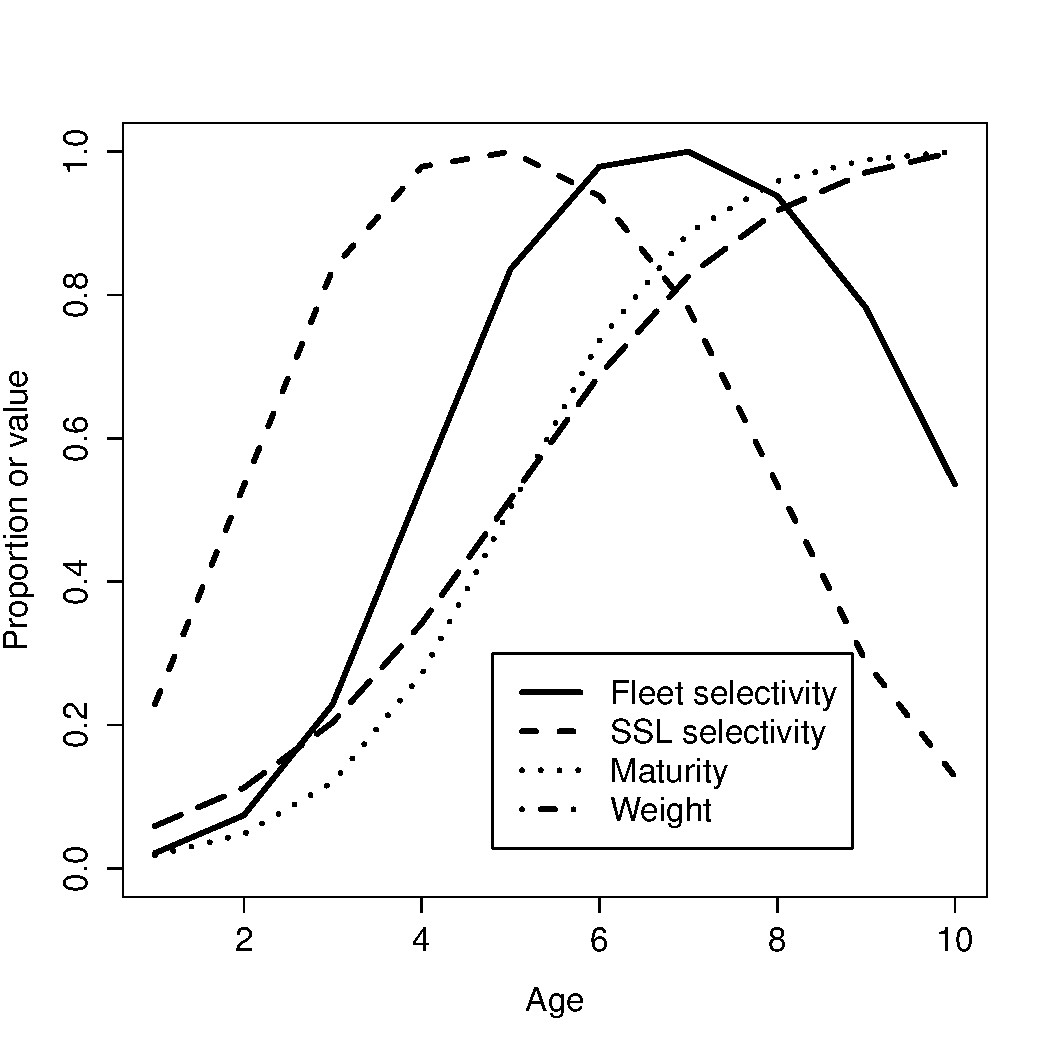
\includegraphics[width= \textwidth]{At_age_plots.pdf}
\end{center}
\caption{A depiction of fishery selectivity-at-age (`Fleet selectivity'), Steller sea lion selectivity (`SSL selectivity'), proportion of sexually
mature fish by age (`Maturity'), and weight-at-age (`Weight'; standardized to have a maximum of 1.0) used
in SSL-fisheries simulation analyses.}
\label{fig:at_age}
\end{figure}

\begin{figure}
\begin{center}
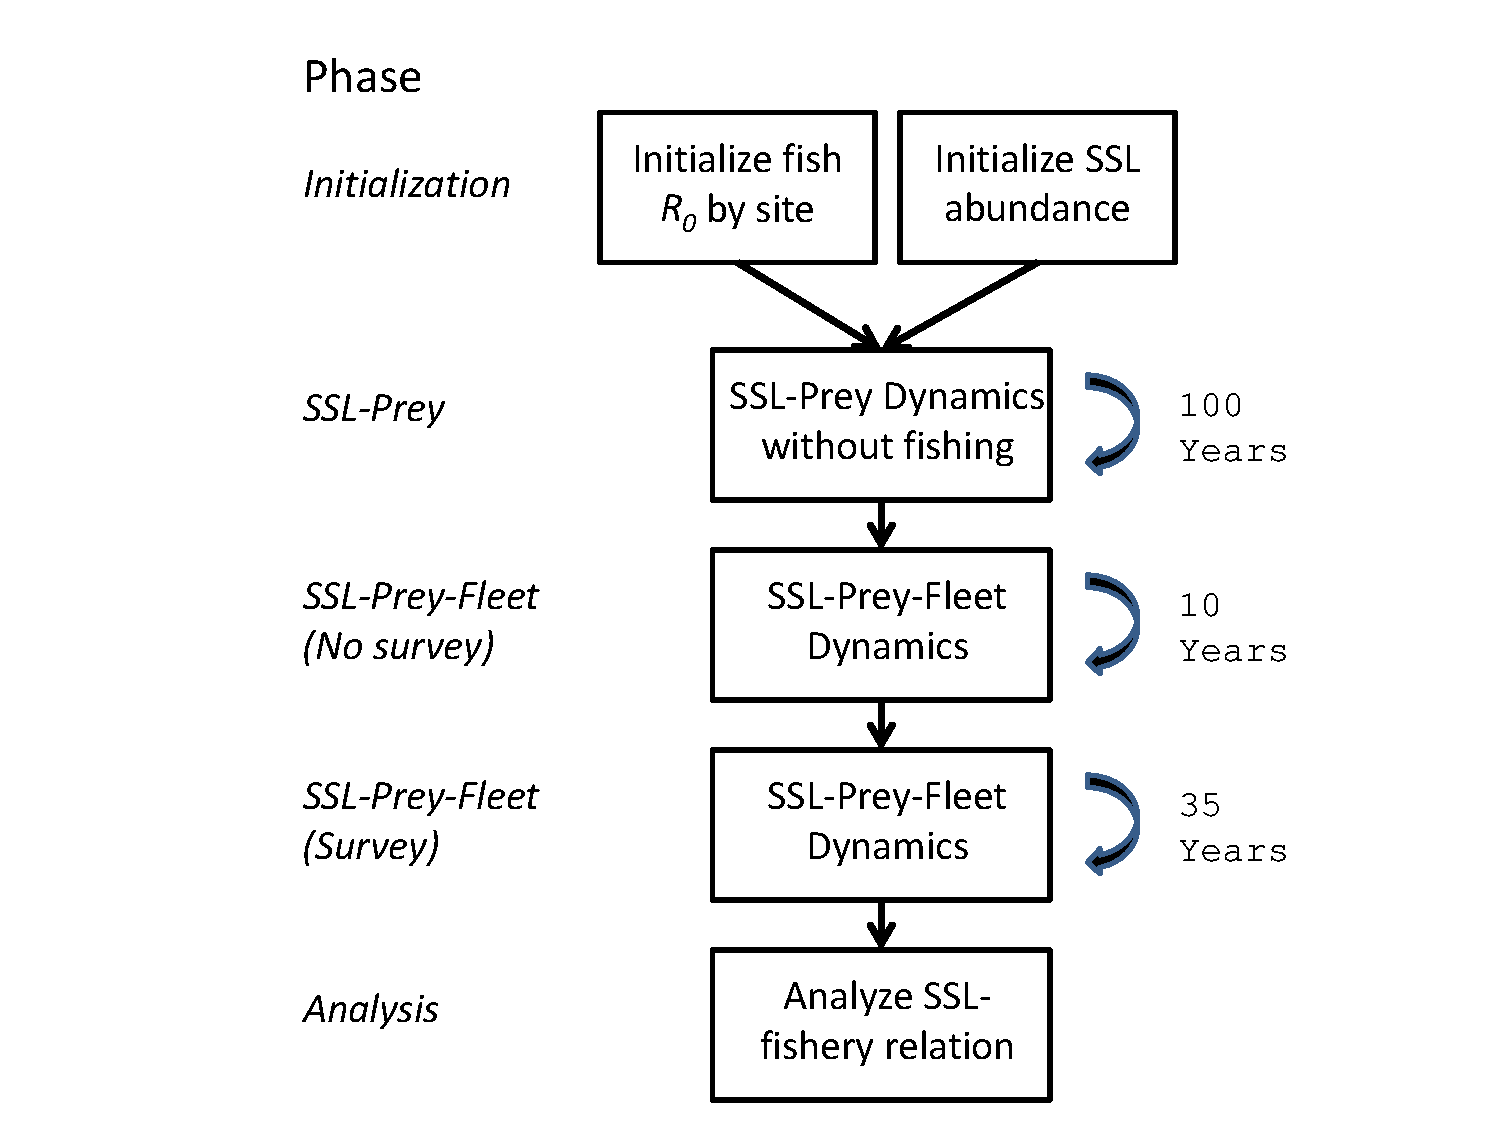
\includegraphics[width= \textwidth]{sim_diagram.pdf}
\end{center}
\caption{A depiction of the simulation structure used in analysis of Steller sea lion (SSL) and fishery
 variables.  At the beginning of each simulation, predator (SSL) and prey (fish) populations are initialized at stable age distributions. After 100 years of simulating predator-prey dynamics to equalize numbers and induce variability in age structure due to fish recruitment stochasticity, fishing is introduced.  Following 10 years of fishing with no survey, simulated aerial surveys are assumed to occur for the next 35 years (at which time catch and CPUE are also calculated).  Finally, after simulated time series are gathered, data are analyzed via generalized linear mixed models to summarize relationships between SSL and fishing variables.}
\label{fig:sim_diagram}
\end{figure}

\begin{figure}
\begin{center}
\includegraphics[width= \textwidth]{sim_trajectories.pdf}
\end{center}
\caption{Examples of simulated SSL time series resulting from calibrated models for SSL, fish, and fishery dynamics.  Five time series are displayed for each simulation scenario, with thin black lines giving total SSL numbers (in 10,000s), and thin grey lines giving scaled fish biomass.  Thick lines represent the mean trajectory over each of the 5 simulations presented.  Top panels (A and B) are representative time series for the case when SSL survival is a function of available fish biomass, while bottom panels (C and D) represent scenarios where available fish biomass affects SSL fecundity.  Left hand panels (A and C) are for cases where fishing effort is randomly allocated among island populations, while right hand panels (B and D) are for cases where fishing effort is allocated proportionally to fish abundance.}
\label{fig:sim_trajectories}
\end{figure}
\end{document}
